\documentclass[11pt]{beamer}
\usepackage[UTF8,scheme=plain]{ctex}
\usepackage{listings}
\usepackage[utf8]{inputenc}
\usepackage[T1]{fontenc}
\usepackage{amsmath}
\usepackage{amsfonts}
\usepackage{amssymb}
\usepackage{graphicx}
\usepackage{txfonts}
\usetheme{Boadilla}

\usepackage{framed} % 可以用 \begin{shaded},即背景色块
\definecolor{shadecolor}{rgb}{0.9,0.9,0.9}

\newcommand{\kong}[1][0.5]{\vspace{#1cm}}

\begin{document}
	\author{ 路毅 \hspace{0.3cm} 曲阜师范大学 }
	\date{\number\year 年 \number\month 月 \number\day 日}
	\title{数学物理方法第三章}

\begin{frame}
	\maketitle
\end{frame}

\kaishu

\begin{frame}{第三章:柯西定理 柯西积分}
\begin{itemize}
	\item 第一节:复变积分的概念及其简单性质
	\vspace{1cm}
	\item 第二节:柯西积分定理及其推广
	\vspace{1cm}
	\item 第三节:柯西积分公式及其推广
\end{itemize}
\end{frame}

\begin{frame}{复变积分}

围线:逐段光滑的闭曲线,正向:“内部”在左侧

\kong[0.5]
复变积分:$C$为起点$z_0$、终点$z^\prime$之间的有向曲线,取$n$个节点$z_0, z_1, \cdots, z_n=z^\prime$,沿正向顺序
\begin{equation}
\Delta z_k = z_k - z_{k-1},
\end{equation}
定义$C$上的复变积分
\begin{equation}
\int_c f(z) dz = \lim_{\Delta z_k \rightarrow 0} \sum^n_{k=1} f(\zeta_k) \Delta z_k,
\end{equation}
其中$\zeta_k$为$z_{k-1}$到$z_k$的弧段上任意一点。
\end{frame}

\begin{frame}{例题1}
试证
\begin{equation}
\oint_C \frac{dz}{(z-a)^n} = \left\{
\begin{aligned}
& 2 \pi i, & n=1 \\
& 0, & n\neq 1, n\in Z
\end{aligned}
\right.
\end{equation}
其中$C$表示以$a$为中心,$\rho$为半径的圆周。

\kong[0.5]
证明:设$z-a=\rho e^{it}$,则有$dz = i\rho e^{it} dt$,
$n=1$时,有
\begin{equation}
\oint_C \frac{dz}{z-a} = \int^{2\pi}_0 \frac{ i\rho e^{it} dt}{\rho e^{it}} = 2\pi i,
\end{equation}
$n\neq 1$,且$n\in Z$时,
\begin{equation}
\oint_C \frac{dz}{(z-a)^n} = \int^{2\pi}_0 \frac{ i\rho e^{it} dt}{(\rho e^{it})^n} = i \rho^{1-n} \int^{2\pi}_0 e^{i(1-n)t}dt = 0,
\end{equation}
\end{frame}

\begin{frame}{例题2}
计算积分$\int_C Re z dz$,其中积分路径$C$如图所示
\begin{itemize}
	\item [(1)] $C$为联结$O$点到$1+i$点的直线段。
	\item [(2)] $C$为联结$O$点到$1$点再到$1+i$点的折线。
\end{itemize}
\begin{figure}
	\centering
	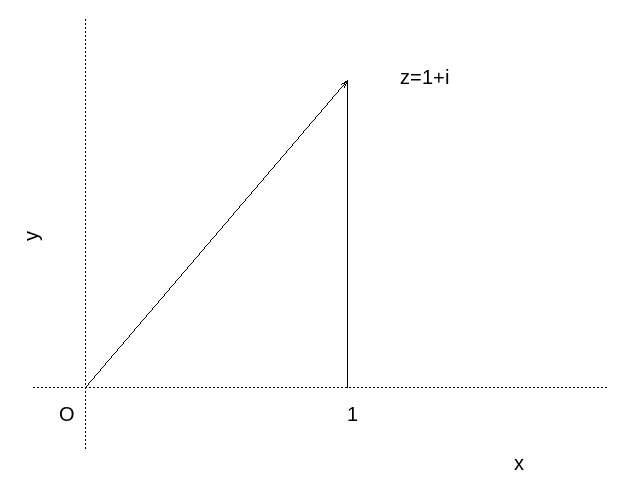
\includegraphics[width=0.7\linewidth]{chap3_example2}
	\caption{例题2}
	\label{fig:chap3example2}
\end{figure}

\end{frame}

\begin{frame}{复变积分的简单性质}

\begin{eqnarray}
\int_C dz &=& z_1 - z_0, \\
\int_C [a_1 f_1(z) + a_2 f_2(z)] dz
 &=& a_1 \int_C f_1(z) dz + a_2 \int_C f_2(z) dz, \\
\int_C f(z)dz &=& \int_{C_1} f(z)dz + \int_{C_2} f(z) dz, C = C_1 + C_2, \\
\int_{C-} f(z) dz &=& - \int_C f(z) dz, \\
|\int_C f(z)  dz| &\leq& \int_C |f(z)| |dz|, \\
|\int_C f(z) dz | &\leq& Ml, 
\end{eqnarray}
其中$M$是$|f(z)|$在$C$上的上界,$l$为$C$的长度。

\end{frame}

\begin{frame}{柯西积分定理}

定理3.1:若$f(z)$在单连通区域$D$内解析,$C$是$D$内的任一围线,则
\begin{equation}
\oint_C f(z) dz = 0.
\end{equation}

若$f^\prime(z)$在$D$内连续,则上述定理很好证明。由于
\begin{equation}
f(z) = u(x,y) + iv(x,y),
\end{equation}
所以有
\begin{equation}
\oint_C f(z) dz = \oint_C udx - vdy + i\oint_C vdx + udy,
\end{equation}
\end{frame}

\begin{frame}{柯西积分定理}
根据格林公式:
\begin{eqnarray}
\oint_C P(x,y)dx + Q(x,y)dy = \oiint_D (\frac{\partial Q}{\partial x} - \frac{\partial P}{\partial y}) dxdy,
\end{eqnarray}
其中$C$为分段光滑曲线,$D$为以$C$为边界的平面单连通区域,$P(x,y)$和$Q(x,y)$在$D$及$C$上连续,并且对$x,y$有连续偏导数\footnote{川大版《高等数学》第二册第四版217页。}。

\begin{eqnarray}
\oint_C f(z) dz &=& \oint_C udx - vdy + i\oint_C vdx + udy, \\
&=& \oint_S (- v_x - u_y)ds + i \oint_S (u_x - v_y) ds, \\
&=& 0.
\end{eqnarray}

\end{frame}

\begin{frame}{不定积分,原函数}
如果$f(z)$的单连通区域$D$内解析,则
\begin{equation}
F(z) = \int^z_{z_0} f(\zeta) d\zeta
\end{equation}
只与起点$z_0$和终点$z$有关,与路径无关。所以选定$z_0$以后,$F(z)$就是关于$z$的函数。其导数为
\begin{equation}
F^\prime(z) = f(z),
\end{equation}
所以$F(z)$称为$f(z)$的不定积分,或原函数。
\end{frame}

\begin{frame}{例题3,4}
例3
\begin{equation}
\int^b_a z \cos z^2 dz = \frac{1}{2}(\sin b^2 - \sin a^2),
\end{equation}

\kong[0.5]
例4
\begin{equation}
\int^z_1 \frac{d \zeta}{ \zeta} = \ln z - \ln 1 = \ln z.
\end{equation}
\end{frame}

\begin{frame}{柯西积分定理:推广到复围线}
\begin{figure}
	\centering
	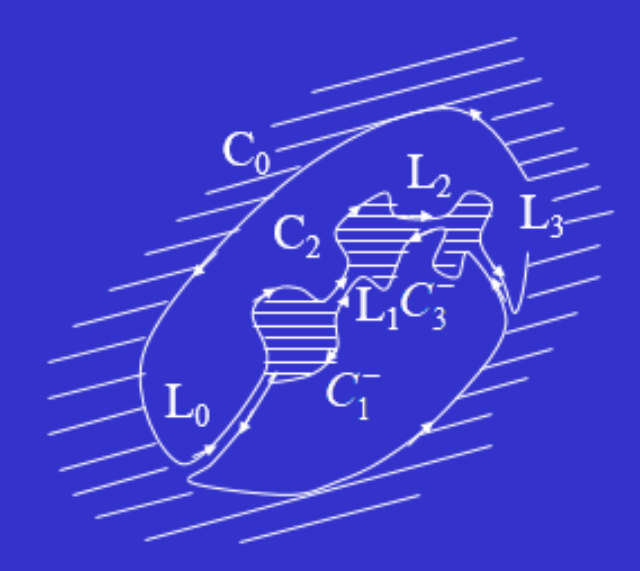
\includegraphics[width=0.5\linewidth]{chap3复围线}
	\caption{复围线上的柯西积分定理}
	\label{fig:chap3}
\end{figure}
如图构造回路,整条回路记为$C$,根据简单围线上的柯西定理有
\begin{equation}
\oint_C f(z) dz = 0,
\end{equation}
\end{frame}

\begin{frame}{柯西积分推广到复围线}
$C$中除了$C_0, C_1, C_2, C_3$以外的部分,在极限情况下抵消,剩下
\begin{equation}
\oint_{C_0} f(z) dz + \oint_{C_1} f(z) dz + \oint_{C_2} f(z)dz + \oint_{C_3} f(z) dz = 0.
\end{equation}
即:解析函数在复围线上的积分为零。
\end{frame}

\begin{frame}{复围线上的柯西积分定理:推论1}
\begin{figure}
	\centering
	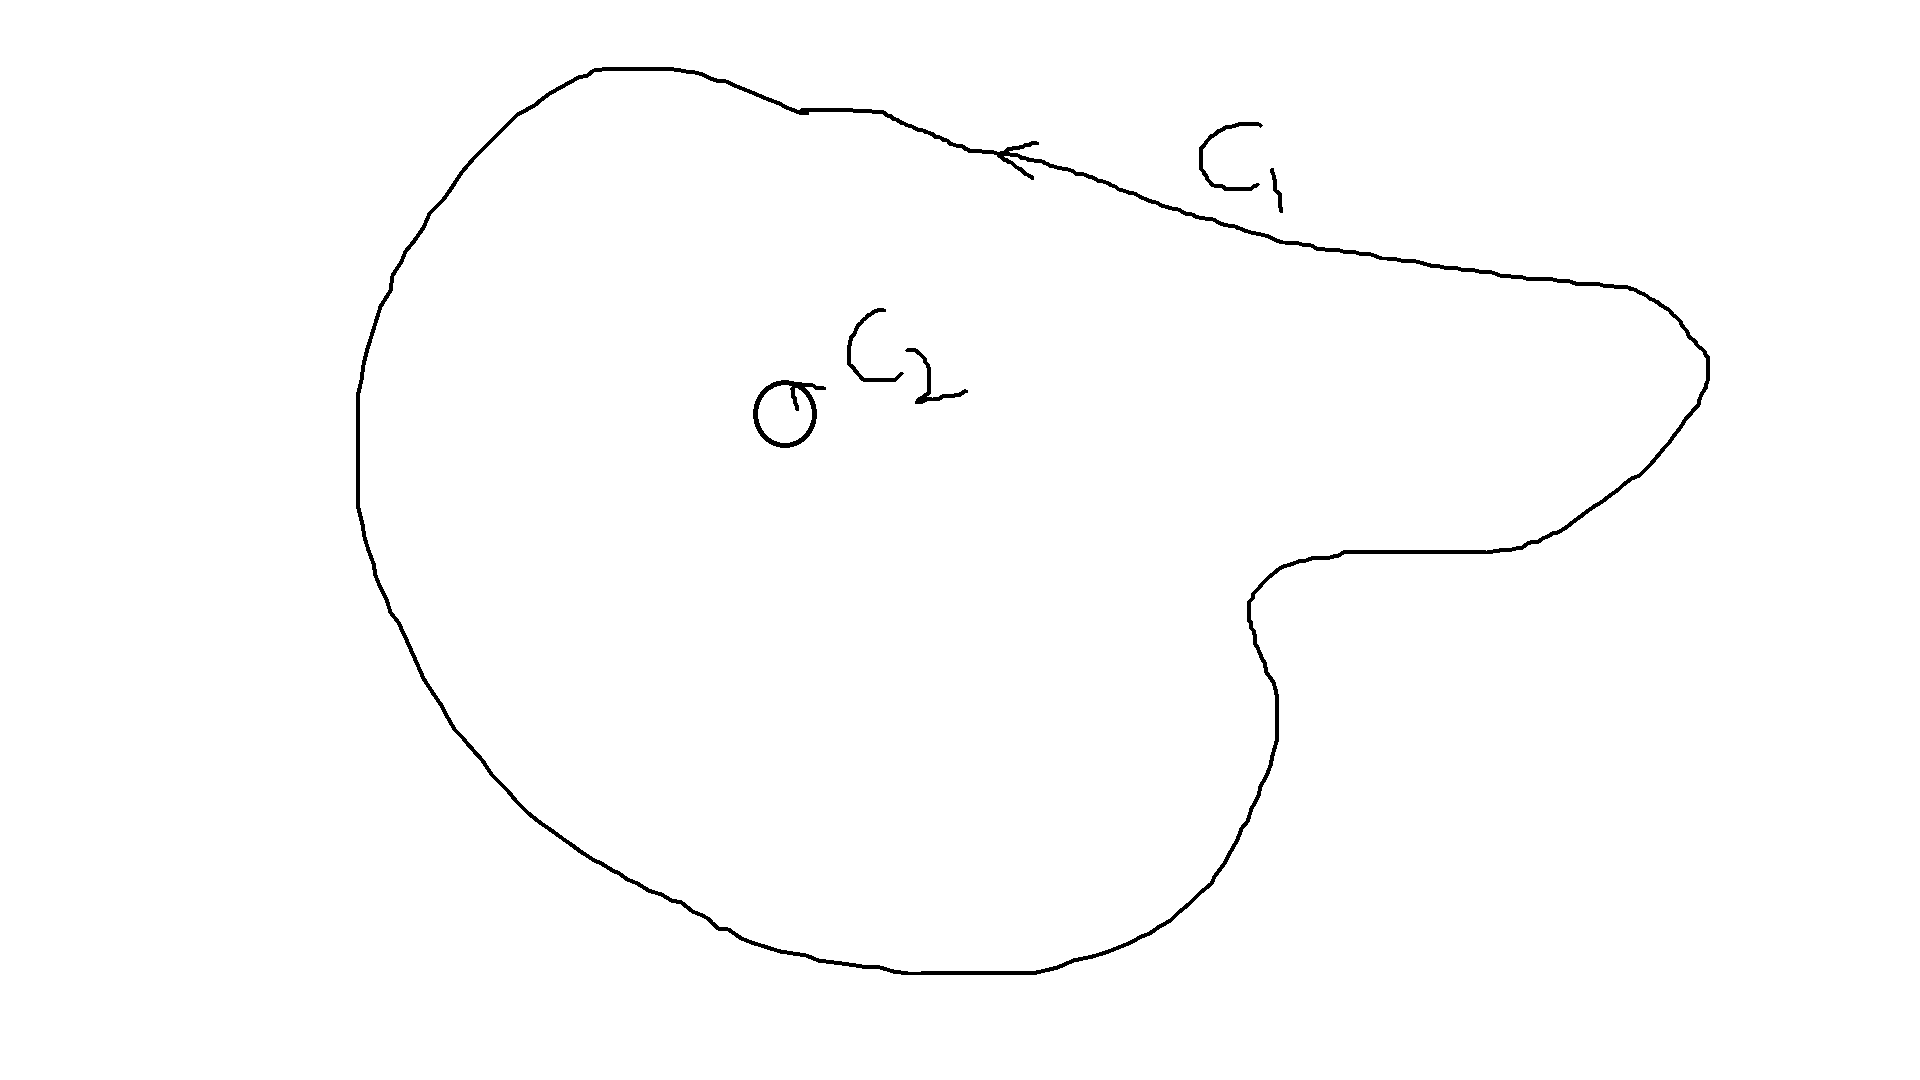
\includegraphics[width=0.5\linewidth]{复围线上的柯西积分定理1}
	%\caption{若$f(z)$在$C_1,C_2$之间的区域解析,则有$\oint_{C_1}f(z) dz = \oint_{C_2}f(z)dz$。}
	\label{fig:1}
\end{figure}
若$f(z)$在$C_1,C_2$之间的区域解析,根据复围线上的柯西积分定理,有
\begin{equation}
\oint_{C_1} f(z) dz + \oint_{C^-_2} f(z) dz = 0,
\end{equation}
其中$C^-_2$与图中$C_2$的方向相反。由于$\oint_{C^-_2} f(z) dz = - \oint_{C_2} f(z) dz$,所以有
\begin{equation}
\oint_{C_1}f(z) dz = \oint_{C_2}f(z)dz.
\end{equation}
\end{frame}

\begin{frame}{复围线上的柯西积分定理:推论2}
\begin{figure}
	\centering
	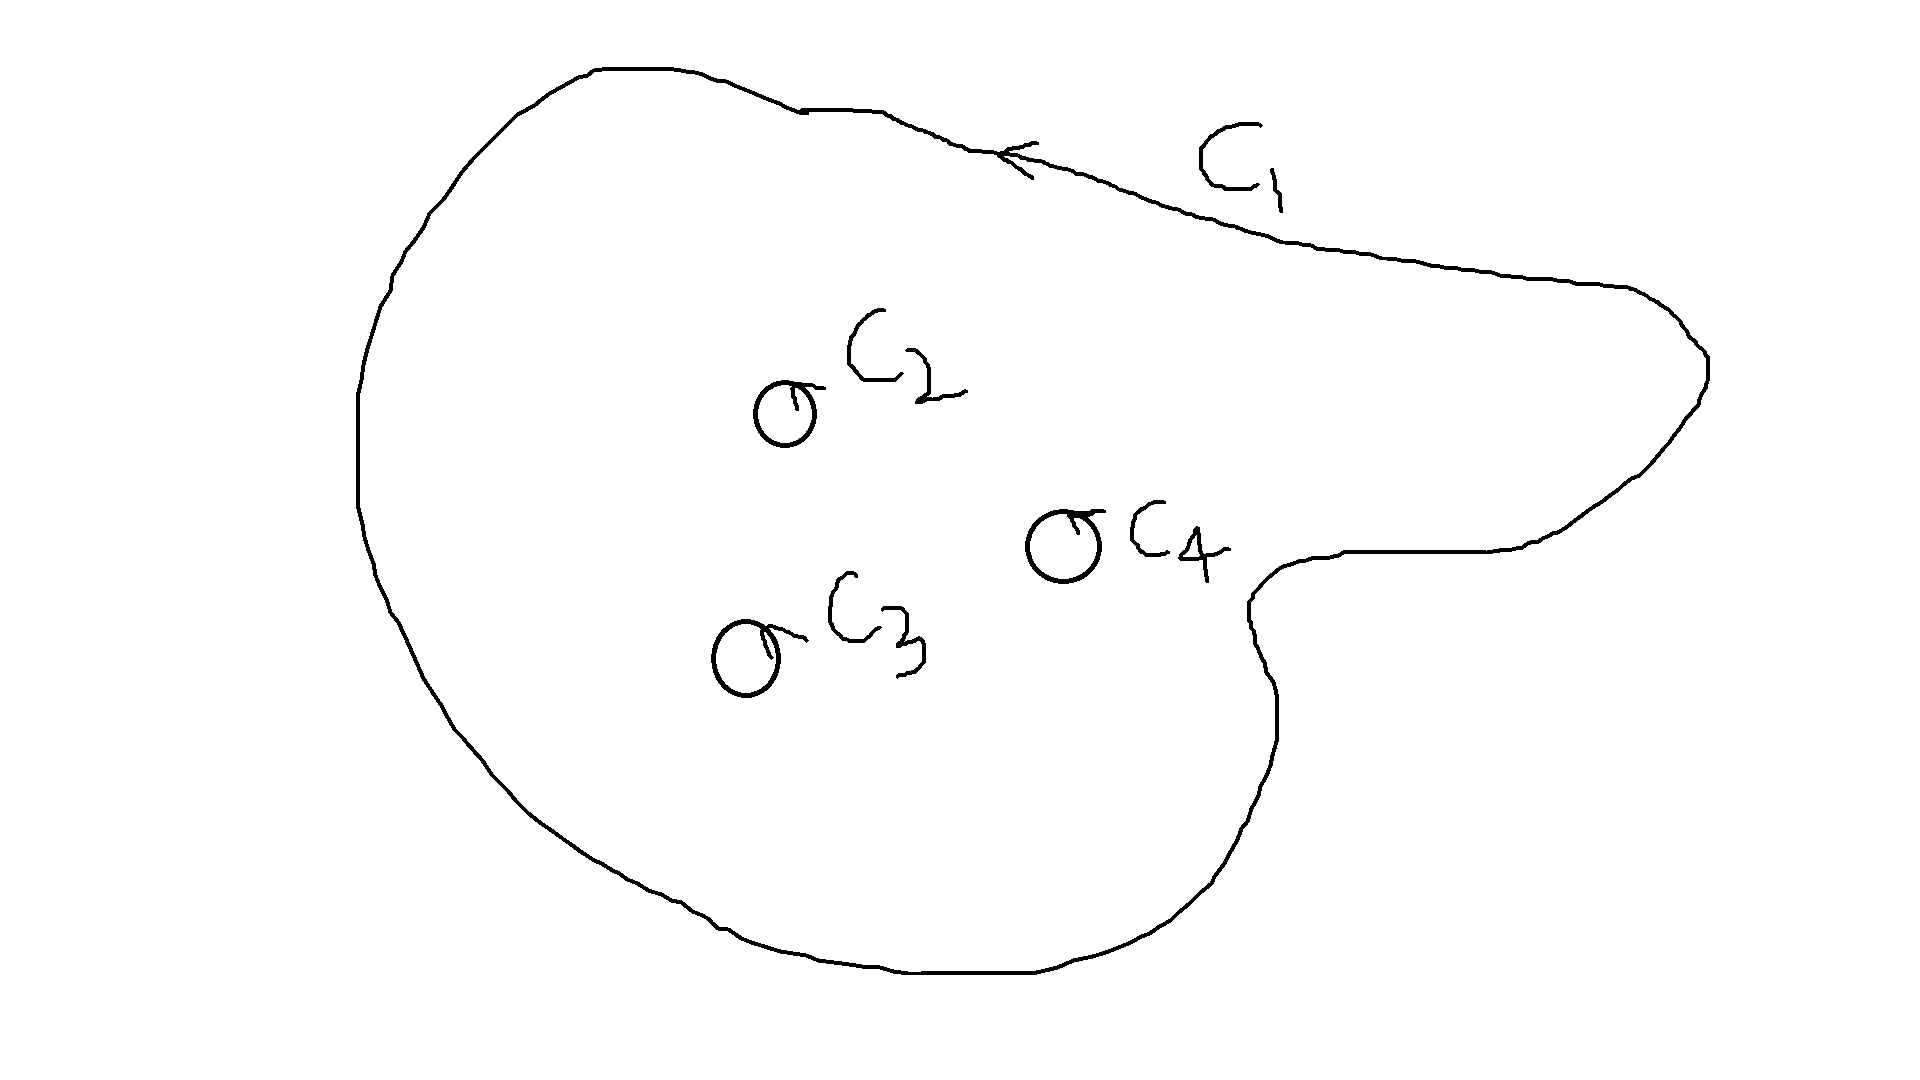
\includegraphics[width=0.5\linewidth]{复围线上的柯西积分定理2}
	%\caption{若$f(z)$在$C_1,C_2$之间的区域解析,则有$\oint_{C_1}f(z) dz = \oint_{C_2}f(z)dz$。}
	\label{fig:2}
\end{figure}
若$f(z)$在$C_1$之内,$C_2,C_3,C_4$之外的区域解析,根据复围线上的柯西积分定理,有
\begin{equation}
\oint_{C_1} f(z) dz + \oint_{C^-_2} f(z) dz + \oint_{C^-_3} f(z) dz + \oint_{C^-_4} f(z) dz = 0,
\end{equation}
所以有
\begin{equation}
\oint_{C_1}f(z) dz = \oint_{C_2}f(z)dz + \oint_{C_3}f(z) dz + \oint_{C_4} f(z) dz.
\end{equation}
\end{frame}

\begin{frame}{例题5}
例5:设$a$是围线$C$内部一点,证明
\begin{equation}
\oint_C \frac{dz}{(z-a)^n} = \left\{
\begin{aligned}
2 \pi i, n=1 \\
0, n \neq 1, n\in Z
\end{aligned}
\right.
\end{equation}

根据前面给出的推论1,
\begin{equation}
\oint_C \frac{dz}{(z-a)^n} = \oint_{\gamma_\rho} \frac{dz}{(z-a)^n},
\end{equation}
其中,$\gamma_\rho$表示以$a$为圆心,以很小的$\rho$为半径($\gamma_\rho$全在$C$内部)的圆。因为$\frac{1}{(z-a)^n}$在$C$与$\gamma_\rho$之间处处解析,所以根据推论1有上面的式子。

可以设$\gamma_\rho$上任意点为$z = a + \rho e^{i\theta}$,则有$dz = i \rho e^{i\theta} d \theta$,所以
\begin{equation}
\oint_C \frac{dz}{(z-a)^n} = \oint_{\gamma_\rho} \frac{dz}{(z-a)^n} = \int^{2\pi}_0 \frac{i \rho e^{i\theta} d \theta}{\rho^n e^{in \theta}}
= \left\{
\begin{aligned}
2 \pi i, n=1 \\
0, n \neq 1, n\in Z
\end{aligned}
\right.
\end{equation}

\end{frame}

\begin{frame}{例题6}
例6:计算$\oint_C \frac{dz}{z^2 -1}$,其中$C$为圆周$|z|=2$。

因为
\begin{equation}
\frac{1}{z^2 -1} = \frac{1}{2}( \frac{1}{z-1} - \frac{1}{z+1} ),
\end{equation}
所以有
\begin{eqnarray}
\oint_C \frac{dz}{z^2 -1} &=& \frac{1}{2}\oint_C \frac{dz}{z-1} - \frac{1}{2} \oint_C \frac{dz}{z+1}
\nonumber\\
&=& \frac{1}{2}(2\pi i) - \frac{1}{2}(2\pi i)
\nonumber\\
&=& 0.
\end{eqnarray}
\end{frame}

\begin{frame}{柯西积分公式}
区域$D$边界是$C$,$f(z)$在$D$内解析,在$\bar{D}=D+C$上连续,则有
\begin{equation}
f(z) = \frac{1}{2\pi i} \oint_C \frac{f(\zeta)}{\zeta - z} d\zeta.
\end{equation}
证明:取$z$为圆心,半径为$\rho$(很小)的回路$\gamma_\rho$,根据复围线的柯西积分定理,
\begin{equation}
\oint_C \frac{f(\zeta)}{\zeta - z} d \zeta
= \oint_{\gamma_\rho} \frac{f(\zeta)}{\zeta - z} d \zeta
= \lim\limits_{\rho \rightarrow 0} \oint_{\gamma_\rho} \frac{f(\zeta)}{\zeta - z} d \zeta = 2\pi i f(z),
\end{equation}
所以有
\begin{equation}
f(z) = \frac{1}{2\pi i} \oint_C \frac{f(\zeta)}{\zeta - z} d\zeta.
\end{equation}
这说明:解析函数的值可以用它在边界上的值表示!可以考虑静电场的唯一性定理。
\end{frame}

\begin{frame}{例7}
回路$C$为圆周$|z|=2$,计算$\oint_C \frac{z}{(9-z^2)(z+i)} dz$。
\begin{equation}
\oint_C \frac{z}{(9-z^2)(z+i)} dz
= \oint_C \frac{z/(9-z^2)}{z-(-i)} dz,
\end{equation}
因为$z/(9-z^2)$在$C$及其内部都解析,所以可以使用柯西积分公式:
\begin{equation}
f(z) = \frac{1}{2\pi i} \oint_C \frac{f(\zeta)}{\zeta - z} d\zeta.
\end{equation}
套用这个公式,计算$z/(9-z^2)$在$z=-i$时的取值,得到
\begin{eqnarray}
\oint_C \frac{z}{(9-z^2)(z+i)} dz
&=& \oint_C \frac{z/(9-z^2)}{z-(-i)} dz,
\nonumber\\
&=& 2\pi i \frac{-i}{9-(-i)^2} = \frac{\pi}{5}.
\end{eqnarray}
\end{frame}

\begin{frame}{解析函数的无限次可微性}
\begin{equation}
f(z) = \frac{1}{2\pi i} \oint_C \frac{f(\zeta)}{\zeta - z} d \zeta, z \in D,
\end{equation}
易得
\begin{equation}
f^{(n)}(z) = \frac{n!}{2\pi i} \oint_C \frac{f(\zeta)}{(\zeta - z)^{n+1}} d\zeta, z \in D, n=1,2,\cdots
\end{equation}
也可以写作
\begin{equation}
\oint_C \frac{f(z)}{(z-a)^n} dz
= \frac{2\pi i}{(n-1)!} f^{(n-1)} (a), a\in D, n=1,2,\cdots
\end{equation}

所以,只要$f(z)$在围线$C$上连续,在$C$内解析,则$f(z)$在$C$内任一点都有任意阶导数,任意阶导数值都可由上式计算,即用$C$上的函数值表达。

\end{frame}

\begin{frame}{例8}
计算积分:
\begin{equation}
I = \oint_C \frac{e^z}{(z^2+1)^2} dz,
\end{equation}
其中$C$是由$|z|=a,a>1$确定的区域。

解:构造复围线,由$C,C_1,C_2$构成,其中,$C_1$为绕$z=i$点的小圆环,$C_2$为绕$z=-i$点的小圆环。根据复围线的柯西积分定理,
\begin{eqnarray}
I &=& \oint_C \frac{e^z}{(z^2+1)^2} dz = \oint_{C_1} \frac{e^z}{(z^2+1)^2} dz + \oint_{C_2} \frac{e^z}{(z^2+1)^2} dz, \nonumber\\
&=& \oint_{C_1} \frac{e^z/(z+i)^2}{(z-i)^2} dz + \oint_{C_2} \frac{e^z/(z-i)^2}{(z+i)^2} dz, \nonumber\\
&=& 2 \pi i [e^z/(z+i)^2]'|_{z=i} + 2\pi i[e^z/(z-i)^2]'|_{z=-i},
\end{eqnarray}
最后一个等号使用了(32)式。所以,经过计算得到
\begin{equation}
I = \frac{\pi}{2}(1-i)e^i + \frac{\pi }{2}(-1-i)e^{-i}
= i\pi \sqrt{2}\sin(1-\pi/4).
\end{equation}
\end{frame}

\begin{frame}{作业}

课堂选讲:1, 4, 5, {\color{blue}7, 8, 15}

\kong[1]
课后作业:2, 9, 11, 12, 14

\end{frame}

\end{document}